% Possíveis TODO
% - expandir nas equacoes xx yy
\documentclass[a4paper,titlepage]{article}
\usepackage[utf8]{inputenc}
\usepackage[T1]{fontenc}
\usepackage[brazil]{babel}
% setspace - \doublespace \onehalfspace
% fullpage - ?? 

\usepackage{verbatim}
\usepackage{url}
\usepackage{hyperref}
\usepackage{graphicx}
\usepackage[bf]{subfigure}
\usepackage[bf]{caption}
\usepackage{amsmath,amssymb}
\usepackage{algorithm,algorithmic}
\usepackage{mathtools,empheq}
\usepackage{macrosfabbri-basic}
\usepackage{macrosfabbri-dg}
\usepackage{xcolor}
\usepackage{ulem}

% ------------------------------------------------------------------------------
% Paper draft Comments and TODO's
%
% You have two versions of the macro
% \draftnote{My note}. The first version puts notes (e.g. My note in the example)
% into the margin of your document. The second formats the note as nothing. You
% 'comment out' the version of the macro you don't want (using a % at the
% beginning of the line).
\newcommand{\draftnote}[1]{\marginpar{\tiny\raggedright\textsf{\textcolor{blue}{\hspace{0pt}#1}}}}
%\newcommand{\draftnote}[1]{}
%
% This one is just for the comments for in-line text.
\newcommand{\indraftnote}[1]{\textcolor{blue}{\texttt{\footnotesize [#1]}}}
\newcommand{\todo}[1]{\indraftnote{todo: #1}} % Este  "a fazer" é para eu não esquecer
\newcommand{\juliana}[1]{\textcolor{red}{#1}}


\begin{document}

\begin{titlepage}
\renewcommand{\title}{%
  {\LARGE Revisão Comentada de Artigo}\\
  \mbox{Barycentric Subspace Analysis on Manifolds}%
}
\renewcommand{\author}{Juliana Santos Barcellos Chagas Ventura\\ Gabriel Andrade}
\renewcommand{\date}{\today}
\newcommand{\info}{%
  \raisebox{4pt}[-4pt]{%
  \includegraphics[height=1.3cm]{figs/logo-iprj.png} 
  \hspace{0.1in}
  }\\

  Instituto Politécnico -- IPRJ\\
  Universidade do Estado do Rio de Janeiro\\[2em]
  
  \includegraphics[height=1.3cm]{figs/logo-ppgmc.png}\\
  Programa de Pós Graduação em Modelagem Computacional\\
  Disciplina de Variedades Diferenciáveis\\
  prof. Ricardo Fabbri\\[1em]

  Nova Friburgo, \date\\[1.5cm]
}

%% Abstand zwischen oberem Blattrand und Titel.
\newlength{\topToTitle} 
\setlength{\topToTitle}{0pt}

%% Abstand zwischen linkem Blattrand und Titel.
\newlength{\leftToTitle} 
\setlength{\leftToTitle}{-60pt}

%% Abstand zwischen Titel und Info-Feld.
\newlength{\titleToInfo} 
\setlength{\titleToInfo}{9.5cm}

%% \myTextWidth erhoehen, um Info-Feld weiter nach Rechts zu schieben.
\newlength{\myTextWidth}
\setlength{\myTextWidth}{\textwidth}
\advance\myTextWidth by 1cm


\thispagestyle{empty}
\vspace*{\topToTitle}
\begin{minipage}{\myTextWidth}
  \sffamily
  \hspace*{\leftToTitle}\begin{minipage}{11cm}
    \Large\textbf{Trabalho final}\\[1.5cm]
    \title\\[1.5cm]
    \author
  \end{minipage}\\

  %% \enlargethispage{} um ggfs. Titel und Info-Feld weiter
  %% auseinanderziehen zu koennen.
  \vspace*{\titleToInfo}

  \begin{minipage}{\textwidth}
    \flushright
    \info
  \end{minipage}
\end{minipage}%
\end{titlepage}


\section{Preliminares}

Este trabalho consiste em expandir o artigo~\cite{Pennec:AnnStat:2018},
cuja primeira página está reproduzida na Figura~\ref{fig:paper:page1}.
O presente texto é uma versão comentada do artigo,
expandindo o máximo possível os conceitos ligados a Variedades Diferenciáveis.
Desta forma, o presente texto é um super-conjunto do referido artigo.
Ele contém todo o artigo, possivelmente em forma de recortes, com expansões e
comentários, e conexões com outros conceitos. Outras referências diretamente
ligadas ao artigo também foram utilizadas para este
trabalho~\cite{Pennec:Advances:Chapter:2020,Sommer:Pennec:etal:2020}.

\begin{figure}
\centering
\frame{\includegraphics[width=0.8\linewidth]{figs/pennec2018-page1.png}}
\caption{% 
Primeira página do artigo sendo revisado. Para baixar, foi necessario o Scihub
pois o portal da CAPES nao continha este periodico apos 2017.
}\label{fig:paper:page1}
\end{figure}

Será utilizada uma mistura de línguas nesta revisão, sendo o inglês preferido
sempre que possível. Sendo assim, não teremos o trabalho de traduzir do inglês
algumas construções básicas do \LaTeX\ como \emph{Theorem} ou
\emph{Definition}.


\section{Tabela de Notação}

This section has a summary of the notation used in the paper, 
mapped to the master notation.

\section{Commented and Expanded Abstract}

Aqui devemos comentar o abstract. Neste caso, escolhemos por comentar
cada parágrafo. Nesta seção, devemos procurar usar linguagem e observações mais
gerais, como se fosse um resumo expandido. Abaixo segue um screen shot do primeiro paragrafo.

{
\vspace{1em}
\frame{\includegraphics[width=0.8\linewidth]{figs/pennec2018-abstract-paragraph1.png}}
\vspace{1em}
}

Variedades Riemannianas podem surgir, por exemplo, no contexto de \emph{data
science}, de um conjunto de dados provenientes de fenômenos não-lineares, em que
os dados possuem uma estrutura de similaridade ou métrica (mais estritamente
falando, de produto interno).

O PCA é uma ferramenta linear das mais importantes para Machine Learning e Data Science.
A extensão do PCA para Variedades Riemannianas pode ser realizada de diversas
formas. A proposta de Pennec~\cite{Pennec:AnnStat:2018,Pennec:Advances:Chapter:2020} é
utilizando os chamados subespaços baricêntricos, construídos através da
geometria de caminhos mínimos, empregando-se geodésicas. Os espaços
baricêntricos generalizam os chamados sub-espaços geodésicos. Com isso,
o PCA generalizado de Pennec se chama \textbf{BSA} (Baricentric Subspace
Analysis). %
\draftnote{BSA: usar esta sigla}%
Barycentric subspaces are implicitly defined
as the locus of weighted means of k + 1 reference points with positive or
negative weights summing up to one. Depending on the definition of the mean, we
obtain the Fréchet, Karcher or Exponential Barycentric subspaces (FBS/KBS/EBS).
Generalizing affine subspaces to manifolds with a minimization procedure (\ie,
Fréchet or Karcher barycentric subspaces) leads to small disconnected patches
that, in the case of constant curvature spaces, do not cover complete lower dimensional subspheres (resp.
sub-pseudospheres). Considering the completion
(the affine span) of all critical points (the exponential barycentric subspace)
is needed to cover the full sub-(pseudo)-sphere~\cite{Pennec:Advances:Chapter:2020}.
\indraftnote{juliana: usar a descricao acima na sua quali}


Pennec afirma que os sub-espaços baricêntricos, por serem 
uma espécie de fecho convexo de pontos de controle, não dependem de vetores
tangentes. Isso permite que as idéias desta generalização do PCA se aplique para
espaços geodésicos que não são Riemannianos.

\begin{question}O que seria um espaço geodésico que não é Riemanniano?
\end{question}
Existem diversas noções ligadas a geodésicas (caminhos mínimos, retas, etc) que
podem se aplicar a espaços que a rigor não são variedades diferenciáveis, como
discretizações~\cite{Video:Geodesics:Crane}, ou a espaços que são variedades
diferenciáveis, porém são não-Riemannianas. É possível que algumas das ideias
de BSA se apliquem a esses casos. Alguns exemplos estão citados na
Seção \ref{sec:discussion} (discussao), como alguns grupos de Lie, que são
naturalmente dotados de uma
conexão bi-invariante e simétrica, mas que pode ser métrica ou não.

\nocite{wikipedia:geodesic:2021}

Se a variedade é diferenciável, as geodésicas estritamente falando precisam
de numa conexão. Escrita em coordenadas, os coeficientes de uma conexão são os
símbolos de Cristoffel, e a equação diferencial da geodésica num ponto e certa
direção é escrita em termos desses símbolos. Se a conexão é consistente com a métrica
Riemanniana, então temos o caso Riemanniano e a conexão se chama Conexão de
Levi-Cività. O caso pseudo- ou semi-Riemanniano
ocorre quando a espécie de métrica imposta na variedade não precisa ser
positiva-definida, ou seja $\langle v,v\rangle \leq 0$ pra algum $v\neq 0$. Mesmo assim, a conexão
pode ser consistente com essa ``pseudo-métrica'' Riemanniana, e nesse caso
a conexão também é a de Levi-Cività. Métricas pseudo-Riemannianas ocorrem em
teoria da relatividade, mas também podem ocorrer em aplicações de machine
learning onde cada dado é representado por um vetor, mas uma das variáveis não é
da mesma natureza das outras e tem pesos diferentes no produto interno, e a
aplicação da teoria é formulada de maneira diferente para esta coordenada.

\begin{remark}
O termo métrica é um termo abusado na literatura, o estritamente correto é que
o tensor ``métrica'' Riemanniano define um produto interno no espaço tangente
(produto interno infinitesimal), e 
o tensor ``métrica'' pseudo ou semi-Riemanniano define algo como produto
interno, mas que não é positivo-definido. Por exemplo, ao fazer esse
``pseudo-produto interno'' numa base de $x$ com ele mesmo, pode-se ter alguns
termos somando outro negando.
If one imposes the positive-definiteness requirement of an inner product on
the metric tensor, this restricts to the case of a Riemannian manifold, and the
path integration yields a metric~\cite{wikipedia:metric:2021}.
\end{remark}



{
\vspace{1em}
\frame{\includegraphics[width=0.8\linewidth]{figs/pennec2018-abstract-paragraph2.png}}
\vspace{1em}
}

O PCA produz um $\mathbb R^k$ (na verdade um espaço afim de dimensão $k$) que
contém os dados, tal que os $k$ eixos (componentes principais) estão ordenados decrescentemente pelo o quanto eles explicam os dados (mais na Seção~\ref{sec:intro} abaixo). Dessa forma, o $\mathbb R^{k-1}$ formado pelos
$k-1$ componentes principais é $\mathbb R^{k-1}$ que melhor explica os dados com
$k-1$ dimensões \juliana{(Não ficaria melhor: ``O espaço afim de dimensão $d=k-1$ formado pelos $k-1$ componentes principais é o espaço afim de dimensão $d$ que melhor explica os dados'')}, no sentido de que a diferença (erro) para usar $k$ dimensões é mínima. Esse erro, estatisticamente falando, é o AUV (accumulated unexplained
variances) referido no abstract. 

Os subespaços baricêntricos são naturalmente encadeados (nested) como o feixo
afim. Imagine em 3D 2 pontos, o fecho convexo seria uma reta; com três pontos o
feixo seria um triângulo (e o plano do triângulo seria o subespaço
baricêntrico, que coincide com subespaço linear \juliana{(linear ou afim?)} 2D); por fim, para um ponto fora do plano, o fecho convexo seria um tetraedro, que seria análogo a um espaço baricêntrico 3D ou o $\mathbb R^3$ no caso de álgebra linear. Dessa forma, o segmento de reta contém os pontos, e a face do triângulo contém as retas e os pontos. Isto é a estrutura hierárquica de \textbf{simplical complex}
ou complexo simplicial. Também nesse sentido os subespaços baricêntricos seriam
análogos a polítopos (polytopes) ou, mais geralmente, poliedros, com a estrutura
hierárquica de flags sendo dada pelo \emph{face lattice}. Conforme o autor
relata mais ao final da introdução, a ordem dos pontos é importante para se
definir quais são os espaços estratificados definidos pelos pontos. Por exemplo,
um quadrado pode ter um dos vértices como sendo mais importante (a ``média''),
um dos lados faces, etc. 

\section{Commented and Expanded Section 1: Introduction}\label{sec:intro}

\begin{center}
\vspace{1em}
\frame{\includegraphics[width=0.8\linewidth]{figs/pennec2018-p1-paragraph1-intro.png}}
\vspace{1em}
\end{center}

Em poucas palavras, o PCA em espaços lineares (afim) pode ser definido
como o menor sub-espaço afim ($\mathbb R^n$ transladado) que contém os dados;
caso uma dimensão $n$ seja especificada, então o PCA de um conjunto é 
o menor sub-espaço afim de dimensão $k$ que capture a máxima variância dos dados
com $k$ dimensões. Se $k$ for maior que a dimensão do espaço que contém os dados
sem erro, então o PCA pode ser calculado sem perda. Se $k$ for menor que esse
valor, então o PCA vai conter perda. Conforme sabemos de Variedades
Diferenciáveis, muitos conjuntos de dados amostrados de fenômenos não-lineares,
por exemplo os provenientes de variedades diferenciáveis ou \emph{manifolds},
não são descritíveis globalmente por um único sistema de coordenadas de dimensão
míninima ou intrínseca. Logo, o PCA na maioria dos casos não-lineares incorre no
problema de ineficiência, pois muitos fenômenos não-lineares não podem ser
descritos de forma global com um único sistema de coordenadas cartesiano com
dimensão igual ao número de grau de liberdades do fenômeno.

Note that it is possible to represent non-manifold areas of a nonlinear dataset
using PCA, it just won't be the minimum linear space or tangent space, but might
have to have larger dimensions. For instance, a 2D cross x might need a 2D space
to be represented using extrinsic coordinates $\mathbb R^2$ (the plane
containing the $x$). So PCA is useful for non-manifold data; it just might not
be the most efficient one. But if one considers it can reduce from 10000
dimensions (say the $x$ represented by a $100\times100$ image) to 2 is already a
the biggest step in terms of compression.

PCA being ``nested'' means that the PCA subspace of dimension $k$ contains the
PCA subspace of dimension $k-1$. That is, the dimensions of the PCA are ordered,
so that if PCA has dimension $n$ then the lower dimensional subspaces that are
``best fit'' for the data are simply the same PCA subspace, but with the lower
dimension removed (the dimension along which the data has least variance). 
 
 \draftnote{As partes que eu, Juliana, acrescentar colocarei em vermelho para facilitar pra mim. Depois tirarei.}
 \juliana{No caso euclidiano, na abordagem \textit{forward} inicia-se com a
 média da amostra para encontrar a primeira autodireção da matriz de
 covariância, que determina a reta que melhor ajusta os dados. O processo segue
 de forma iterativa resultando numa sequência de espaços afins que melhor
 ajustam os dados, "nested" em ordem crescente de dimensão. Já na abordagem
 \textit{backward}, inicia-se com o melhor espaço afim de dimensão r que ajusta
 os dados. Dentro dele procura-se o melhor espaço afim de ajuste de dimensão
 r-1, etc. O que também resulta em uma sequência dos melhores espaços de ajuste,
 indexados pela dimensão. pelo teorema de Pitágoras, ambas as abordagens
 resultam na mesma sequência de espaços afins. Porém, em espaços não euclidianos
 a igualdade das sequências não se verifica~\cite{Damon:Marron:JMIV2014}.}
 
{
\vspace{1em}
\frame{\includegraphics[width=0.8\linewidth]{figs/pennec2018-p1-paragraph2-intro.png}}
\vspace{1em}
}
\draftnote{Revisar aqui a media de Fréchet e também rapidamente o Karcher mean}

Neste trecho, o autor nos informa as condições as quais devemos ter para que tal
generalização seja feita. Uma delas é que definamos um equivalente a subespaços
afins em termos de variedades. Primeiramente o que é um espaço afim? Um espaço
afim é definido informalmente como um espaço que não possui uma origem definida.

\juliana{Seja $V$ um espaço vetorial. $W \subset V$ é um subespaço afim de V se
existir um vetor $w_0 \in V$ e um subespaço vetorial $V_0 \subset V$ tal que
$W=\{w_0 +v ; v \in V_0 \}$.} \juliana{Se $V=\mathbb{R}^2$ ou $V=\mathbb{R}^3$,
o subespaço afim W é o subconjunto obtido da translação do subespaço vetorial
$V_0$ (que por definição passa pela origem (0,0) ou (0,0,0), respectivamente) de
modo que a origem esteja em $w_0$, ou seja, W é um subconjunto "paralelo'' a
$V_0$ que passa pelo ponto $w_0$.}

Pode-se dizer também, segundo o autor, que para um espaço de dimensão zero, ou
seja, um espaço discreto, \draftnote{Gabriel's comment: link de onde tirei isso
\url{https://encyclopediaofmath.org/wiki/Zero-dimensional_space}} uma abordagem
com o uso da média de Fréchet no conjunto da minima da variança é naturalmente
pensada quando aborda-se o problema em termos de variedades. A média de Fréchet
é uma generalização aos centróides, onde é encontrado um ponto em um conjunto de
pontos que possa melhor representar a tendência dos mesmos no grupo.  Em termos
de variedades, supondo que tenhamos uma nuvem de pontos discretos dentro de uma
variedade, o uso da média de Fréchet nos ajudaria a encontrar a
tendencia desta nuvem, proporcionando uma melhor escolha de componentes pela
PCA. \draftnote{Gabriel's comment: Foi pelo menos o que eu a principio entendi
deste trecho}

\juliana{A média de Fréchet é uma generalização da média aritmética em espaços
métricos abstratos e, em geral, não é única (Ginestet, Simmons, Kolaczyk,
2012).}
Em termos estatísticos,
\juliana{
um ponto $\mu$ em um espaço métrico \textbf{M} com função distância $\rho$ é
chamado de média de Fréchet da variável aleatória $X$ em \textbf{M} se satisfaz
$\mu=arg \min \limits_{x \in M} E[\rho(x,X)^2]$.}

\begin{center}
\vspace{1em}
\frame{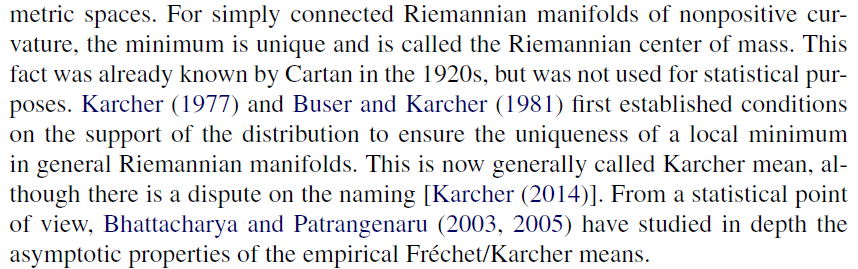
\includegraphics[width=0.8\linewidth]{figs/pennec2018-karcher.PNG}}
\vspace{1em}
\end{center}

\juliana{Se \textbf{M} é uma variedade riemanniana, ela é localmente homeomorfa
(na verdade, difeomorfa em um sentido preciso) a um espaço euclidiano e as
distribuições limites para as médias de Fréchet das amostras são, em geral,
gaussianas; fenômeno semelhante ao das médias euclidianas (LE, H. 2015). A
curvatura seccional de uma superfície é uma generalização da curvatura
gaussiana; assim, se a curvatura gaussiana é negativa, então a curvatura
seccional também é. Portanto, em uma variedade Riemanniana completa,
simplesmente conexa e de curvatura seccional não-positiva a média de Fréchet é
única (POLANÍA, 2014). A média de Frechét é considerada uma média global,
enquanto médias locais de medidas de probabilidade em variedades riemannianas
são  chamadadas de médias de Karcher (ARNAUDON, BARBARESCO,YANG.  2011)}
\draftnote{Juliana's comment:Explicar melhor}

Ver mais sobre médias de Frechet e Karcher
em~\cite{Pennec:Advances:Chapter:2020}.


\begin{center}
\vspace{1em}
\frame{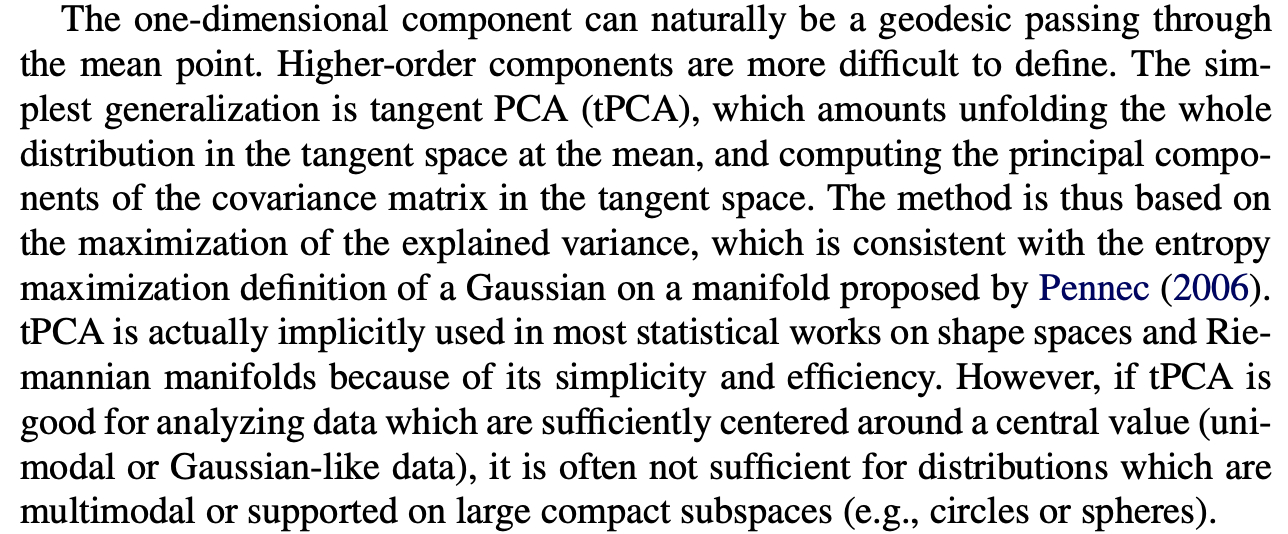
\includegraphics[width=0.8\linewidth]{figs/pennec2018-tPCA.png}}
\vspace{1em}
\end{center}

\begin{center}
\vspace{1em}
\frame{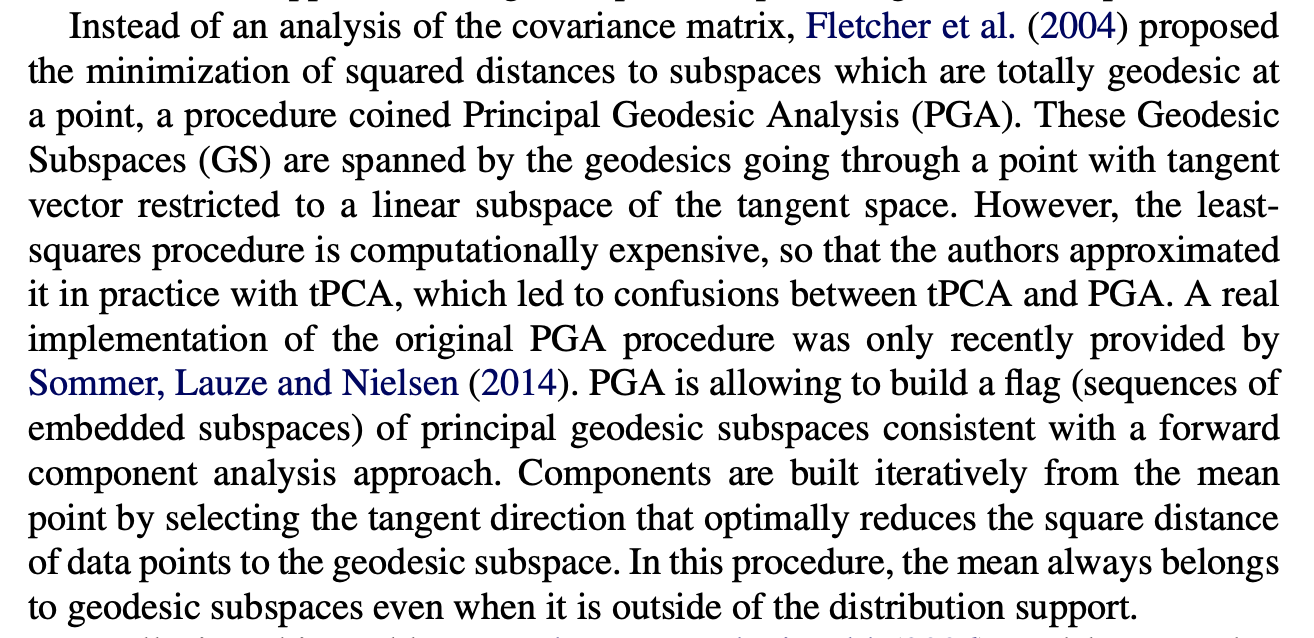
\includegraphics[width=0.8\linewidth]{figs/pennec2018-PGA.png}}
\vspace{1em}
\end{center}

Se a média de Frechet seria análogo ao ``subespaço principal''  de dimensão 0
(origem) do PCA, então os subespaços de dimensão 1, 2, 3, seriam naturalmente
ancorados nessa média. Para definir esses espaços, podemos utilizar a estrutura
de espaço vetorial induzida pelo espaço tangente nos caminhos da variedade que passam por esse ponto
médio. Através do mapa exponencial, a estrutura de espaço vetorial de caminhos
lineares passando pela origem (vetores) do plano tangente, é induzida nos caminhos
não-lineares da variedade, consistindo de geodésicas. Nessa estrutura, é
possível somar caminhos, somando-se os vetores tangentes no plano tangente.
De certa forma, essa soma vira multiplicação de caminhos, pois o mapa
exponencial de uma soma de vetores tangentes é a multiplicação de caminhos.
Logo, se pegarmos todas as combinações lineares de dois vetores fixos em um espaço
tangente de uma variedade 3D, podemos formar um sub-espaço geodésico 2D que tem
uma estrutura subjacente de espaço vetorial, assim como no caso do PCA linear.
Em outras palavras, é possível somar caminhos e multiplicar por escalar através
dos mapas exp e log.
\draftnote{fabbri: elaborar}


\section{Commented and Expanded Section 2: Riemannian geometry}

\begin{center}
\fbox{\parbox[c]{11cm}{In statistics, directional data occupy a place of
choice [Dryden (2005), Huckemann and Ziezold (2006)]. Hyperbolic spaces are
also the simplest models of negatively curved spaces which model the space of
isotropic Gaussian parameters with the Fisher–Rao metric in information geome-
try [Costa, Santos and Strapasson (2015)]. As nonflat constant curvature spaces,
both spherical and hyperbolic spaces are now considered in manifold learning for
embedding data [Wilson et al. (2014)]. Thus, they are ideal examples to illustrate the theory throughout this paper.}}
\end{center}

Neste trecho, o autor nos revela neste parágrafo que em termos de simplicidade,
ele escolhe duas abordagens que são as "dados direcionais'' e os espaços
hiperbólicos. Os chamados dados direcionais se referem a uma formulação
relativamente recente da estatística conhecida como estatística direcional. Essa
formulação trata de dados direcionais, como rotações, em especial estatística em 
espaços Riemannianos compactos. Mais tarde, com as
figuras, veremos que o autor utiliza os dados da PCA em uma distribuição
circular.\draftnote{Gabriel's notes: checar se está correto e reescrever.
Preciso entender melhor este processo. Uma reunião talvez...} 

\juliana{Os espaços esférico e hiperbólico são exemplos de espaços pseudo-euclidianos, isto é, espaços cujas dimensões são caracterizadas por autovalores negativos e a distância quadrada entre objetos tem componentes positivos e negativos que são somados para fornecer a distância total. Espaços pseudo-euclidianos não são métricos, o que dificulta calcular corretamente propriedades geométricas. Uma alternativa é imergir os dados em uma variedade curva, que é um espaço métrico, mas não euclidiano (WILSON, \textit{et all}, 2014).}
\draftnote{juliana: esta estranho, espaco esferico com autovalores negativos?
talvez esteja misturado aqui}

Os espaços hiperbólicos são escolhidos por serem espaços homogêneos onde a curvatura do espaço é a curvatura do espaço seccionado; \juliana{ela é constante e negativa. Já a curvatura dos espaços esféricos é constante e positiva}.
\sout{Uma comparação com o espaço euclidiano, enquanto o simples é utilizando um triângulo construído no espaço euclidiano e no espaço hiperbólico, no espaço euclidiano, a soma dos ângulos "S=180$^{\circ}$'' no hiperbólico "S<180º''.} 
\draftnote{Juliana's comment: a parte riscada achei desnecessária. O que acha?}

\begin{center}
\fbox{\parbox[c]{11cm}{\textit{Tools for computing on Riemannian manifolds.} We consider a differential manifold M endowed with a smooth scalar product  $\langle | \rangle$ called the Riemannian metric on each tangent space $T_x M$ at point x of M. In a chart, the metric is specified by the dot product of the tangent vector to the coordinate curves: $gij (x) = \langle \partial i | \partial j \rangle_{x}$ . The Riemannian distance between two points is the infimum of the length of the curves joining these points. Geodesics, which are critical points of the energy functional, are parametrized by arc-length in addition to optimizing the length. We assume here that the manifold is geodesically complete, that is, the definition domain of all geodesics can be extended to $\mathbb{R}$. This means that the manifold has no boundary nor any singular point that we can reach in a finite time. As an important consequence, the Hopf–Rinow–De Rham theorem states that there always exists at least one minimizing geodesic between any two points of the manifold (i.e., whose length is the distance between the two points).}}
\end{center}

Neste trecho o autor começa a nos mostrar o ferramental usado para o artigo. Primeiramente ele \sout{define} \juliana{considera} uma variedade \juliana{diferencial} $M$ com um produto escalar suave, conhecido como métrica Riemmaniana no espaço tangente $T_{x}M$ em um ponto $x$ de $M$.

\juliana{Se $\textbf{u}:U \subset\mathbb{R}^n \rightarrow M$ é um sistema de coordenadas locais em torno de $x$, com $\textbf{u}=(u_1, ..., u_n)=q \in \textbf{u}(U)$ e $\frac{\partial}{\partial u_i}(q)= d \textbf{u}(0,...,1...,0)$, então $\langle \frac{\partial}{\partial u_i}(q), \frac{\partial}{\partial u_j}(q)\rangle_q = g_{ij}(u_1,...,u_n)$ é uma função diferenciável em $U$ (CARMO, 2015)} \sout{e em seguida ele constrói uma função $g(x)$ tal que $g_{ij}(x)=\langle \partial_i | \partial_j \rangle $.} Isso significa que $g_{ij}(x)=||\partial_i||,i=j$, $g_{ij}(x)=\sum (\partial_i \partial_j)^2,i\neq j$, o que representa a derivada direcional. \draftnote{Juliana comment's: No caso particular do produto interno usual em $R^n$, acho que coincide com a derivada direcional, mas acho que não se aplica para qualquer produto interno. Do Carmo não usa produto escalar, mas produto interno (seção 2, capítulo 1).} 
\\Na sequência, o autor descreve as geodésicas como parametrizações dos comprimentos de arco que otimizam esses comprimentos \sout{a partir disso, constrói uma geodésica parametrizando pelos ótimos de $g$}; e, como ele assume que esta variedade é geodesicamente completa, ele consegue atribuir uma correlção da variedade ao espaço $\mathbb{R}$ chegando a condlusão que a variedade não possui nem ponto de singularidade nem contorno que possa-se chegar em um tempo fnito e, por fim, que o Teorema de Hopf-Rinow-De Rham é satisfeito. \draftnote{Gabriel: Escrever melhor essa parte}

\vspace{1em}
\frame{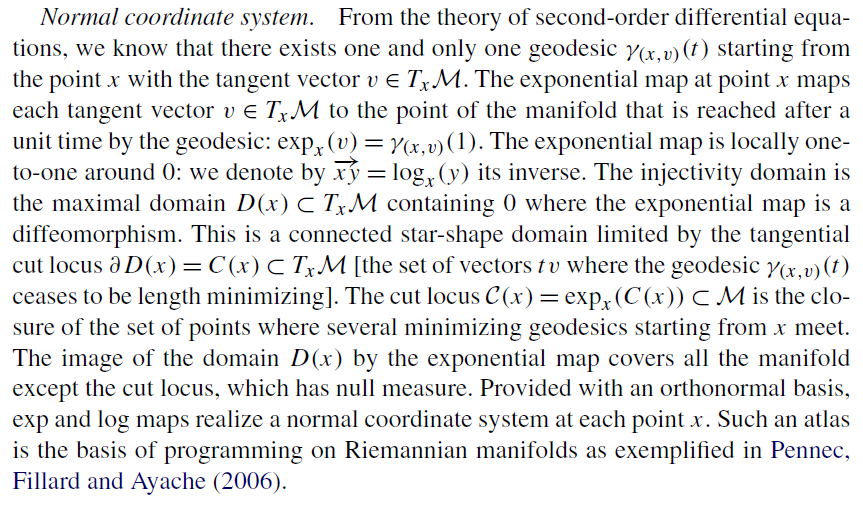
\includegraphics[width=0.95\linewidth]{figs/pennec2018-cutlocus.PNG}}
\vspace{1em}

\juliana{Neste parágrafo o autor introduz o mapa exponencial $exp_x(v)$, que mapeia cada vetor $v \in T_xM$ em um ponto na variedade, obtido após 1 unidade de tempo pela geodésica, isto é, $exp_x(v)=\gamma(x,v)(1)$. O mapa exponencial é um difeomorfismo local numa vizinhança de 0, sendo sua inversa: $\overrightarrow{xy}=\log_x y = v \in T_xM$.}


\juliana{Se $M$ é uma variedade riemanniana completa e $\gamma (x)$ uma geodésica normalizada, com $\gamma (0)=x$, para $t>0$ e suficientemente pequeno, $d(\gamma (0), \gamma (t))=t$, ou seja, $\gamma ([0,t])$ é uma geodésica minimizante. Se existe $t_1$ tal que $d(\gamma (0), \gamma (t_1))>t$, então para todo $t\geq t_1$ a geodésica não é minimizante. Deste modo, se $d(\gamma (0), \gamma (t))=t$ no intervalo $[0,t_0]$, então $\gamma (t_0)$ é chamado de ponto mínimo de $x$ ao longo de $\gamma$.}
\juliana{O conjunto $C(x) \in T_xM$, chamado de \textit{tangential cut locus}, é o conjunto dos vetores $tv$ onde a geodésica $\gamma(x,v)(t)$ deixa de ter comprimento mínimo. Assim, o \textit{cut locus} de $x$ (ou local dos pontos mínimos de $x$), $\mathcal{C}(x)= exp_x(C(x)) \subset M$, é a união dos pontos mínimos de $x$ ao longo de todas as geodésicas que partem de $x$ (do CARMO, 2015). Ou, como escreve o autor, é o fecho do conjunto de pontos onde várias geodésicas minimizantes iniciando em $x$ se encontram.}

\begin{center}
\fbox{\parbox[c]{11cm}{DEFINITION 1 ((k+1)-pointed/punctured Riemannian manifold). 
\\
\textit{Let ${x_0,...,x_k} \in \mathcal{M}^{k+1}$ be a set of $k + 1$ reference points in the n-dimensional Riemannian manifold $\mathcal{M}$ and $C(x_0,...,x_k) = \bigcup_{i=0}^{k} C(x_i)$ be the union of the cut loci of these points. We call the object consisting of the smooth manifold $\mathcal{M}$ and the $k + 1$ reference points a $(k + 1)$-pointed manifold. Likewise, we call the submanifold $\mathcal{M}^{*}(x_0,...,x_k) = \mathcal{M} \ C(x_0,...,x_k)$ of the non-cut points of the $k + 1$ reference points a $(k + 1)$-punctured manifold.}}}
\end{center}

\begin{center}
\fbox{\parbox[c]{11cm}{On $\mathcal{M}{*}(x_0,...,x_k)$, the distance to the points ${x0,...,xk}$ is smooth. The Riemannian log function $\vec{x x_i} = \log_x(x_i)$ is also well defined for all the points of $\mathcal{M}{*}(x_0,...,x_k)$. Since the cut locus of each point is closed and has null measure, the punctured manifold $\mathcal{M}{*}(x_0,...,x_k)$ is open and dense in $\mathcal{M}$, which means that it is a submanifold of $\mathcal{M}$. However, this submanifold is not necessarily connected.
For instance in the flat torus $(S_1)^n$, the cut-locus of $k + 1 \leq n$ points divides the torus into kn disconnected cells.}}
\end{center}

Nesta definição, o autor essencialmete começa a com a definição de um conjunto de $k+1$ pontos da variedade, que pode ser um conjunto de dados quaisquer e $C(x_0,x_1,...,x_k) =\bigcup_{i=0}^{k} C(x_i)$ como ele diz, é \sout{o corte local} \juliana{a união dos \textit{cut loci} ou locais dos pontos mínimos} desse conjunto de dados.
\sout{O \juliana{\textit{cut locus}} é um conjunto de vetores nos espaço tangente da variedade que minimizam o mapeamento exponencial (Esta minimização é dada pela distância geodésica) em torno de um ponto. Com isso $C(x_0,x_1,...,x_k)$ pode ser interpretado como}
Em seguida ele cria uma subvariedade $\mathcal{M}{*}$ que pega todos os pontos que não fazem parte dos mínimos locais da base de dados e que a distância dos pontos pertencentes a ela e dos $x_i$ é suave. Ele diz que o mapeamento logaritmico é bem definido em $\mathcal{M}{*}$, por consequencia desta suavidade. Ele apresenta que o corte local em cada ponto $x_i$ eh um conjunto fechado e tem medida nula, $\mathcal{M}{*}$ eh aberto e denso na variedade, provando que eh uma subvariedade em $\mathcal{M}$. O corte local eh um conjunto fechado devido a sua definicao e ela  

\vspace{1em}
\frame{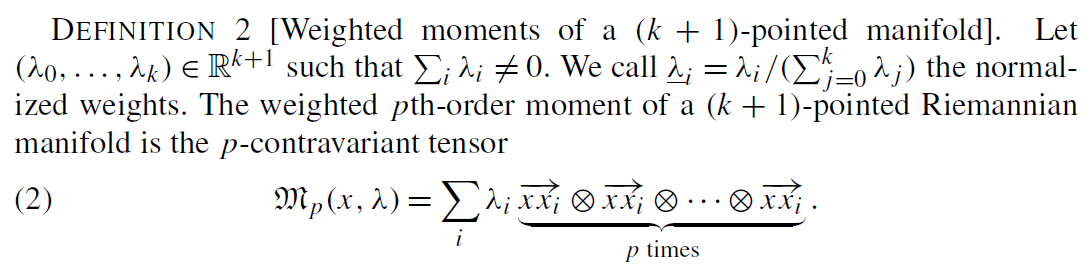
\includegraphics[width=0.95\linewidth]{figs/pennec2018-def2.PNG}}
\vspace{1em}

Na definicao 2 o autor define um conjunto de pesos $\lambda_i \in \mathbb{R}{k+1}$ tais que soma de todos os elementos seja diferente de 0 e tambehm um peso normalizado e define que o momento de peso de p-esima ordem de uma variedade de $k+1$ pontos eh dada pela equacao 2. Vale notar que essa momento p eh uma metrica Riemmaniana de ordem p, semelhante a norma-p no espaco euclidiano.
\begin{center}
 \fbox{\parbox[c]{11cm}{DEFINITION 3 (Affinely independent points). A set of $k + 1$ points ${x_0,...,x_k}$ is affinely independent if no point is in the cut-locus of another and if all the sets of $k$ vectors ${\log_{x_i}
(xj)}_{0\leq j\neq i \leq k} \in T_{x_i}\mathcal{M}^k$ are linearly independent.}}
\end{center}

Esta definicao e simplesmente o fato de que se temos $k+1$ dados no meu conjunto de dados,sao pontos "afinamente" independentes se eles nao possuirem minimo local comum e possamos construir um mapeamento logaritmico, cuja a base sao os conjuntos de vetores em que o mapeamento logaritmico pertence ao plano tangente da variedade
\section{Commented and Expanded Section 3: Exponential Barycentric Subspaces
(EBS) and affine spans}
{
\vspace{1em}
\frame{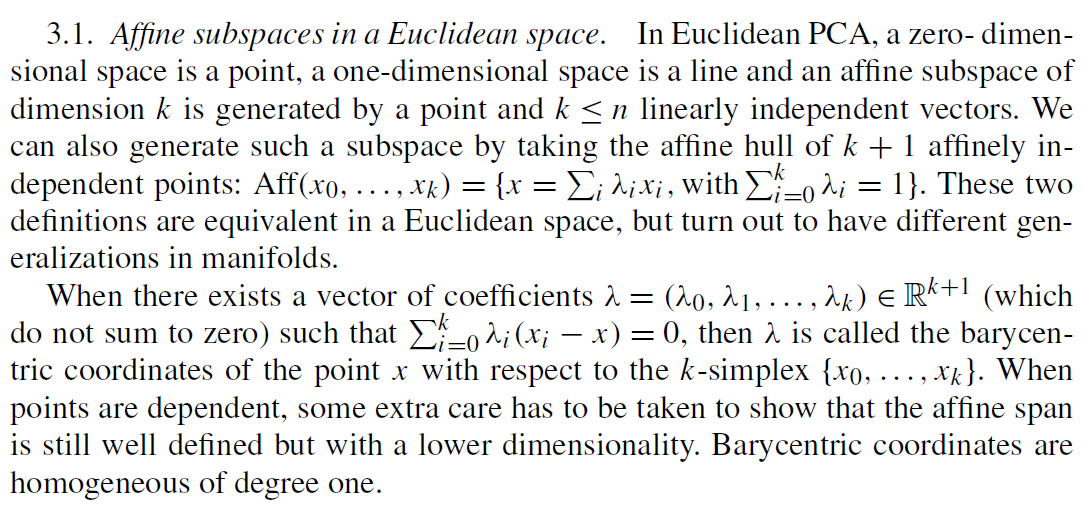
\includegraphics[width=1\linewidth]{figs/pennec2018-sec3-1.PNG}}
\vspace{1em}
}

\juliana{No primeiro parágrafo o autor define de duas formas diferentes, mas equivalentes, subespaços afins em espaços euclidianos e destaca que a equivalência não verifica para variedades.}

\juliana{Podemos dizer que os coeficientes $\lambda_i's$ da definição de Aff$(x_0 ,..., x_k)$ (que chamaremos de $\underline{\lambda}_i$) estão normalizados, enquanto os $\lambda_i's$ da coordenada baricêntrica não necessariamente. O vetor $\lambda$ é múltiplo escalar do vetor $\underline{\lambda}$.} 

\juliana{O $k$-simplex dos pontos $x_0, ..., x_k$ afins independentes (dimensão de Aff$(x_0 ,..., x_k)$ é $k-1$) é o conjunto de todas as combinações afins $\sum_{i=0}^k \lambda_i x_i$, com $\sum_{i=0}^k \lambda_i=1$, tais que $\lambda_i \geq 0$ (fecho convexo).}

{
\vspace{1em}
\frame{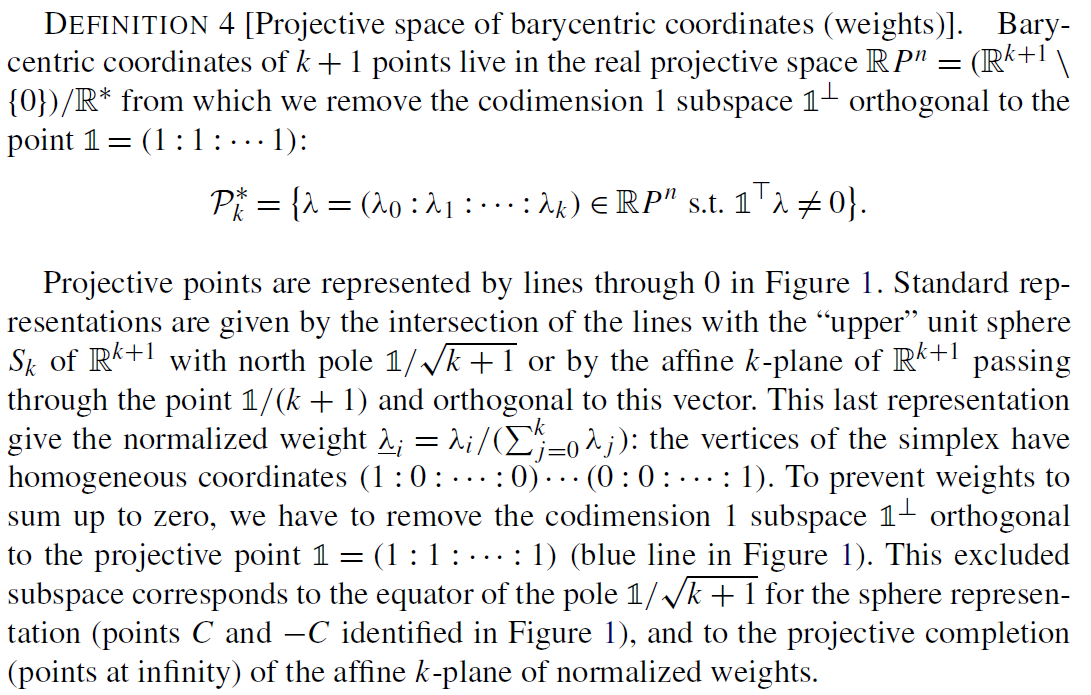
\includegraphics[width=.9\linewidth]{figs/pennec2018-def4.PNG}}
\vspace{1em}
}

\section{Commented and Expanded Section 4: Fréchet/Karcher barycentric subspaces}
{
\vspace{1em}
\frame{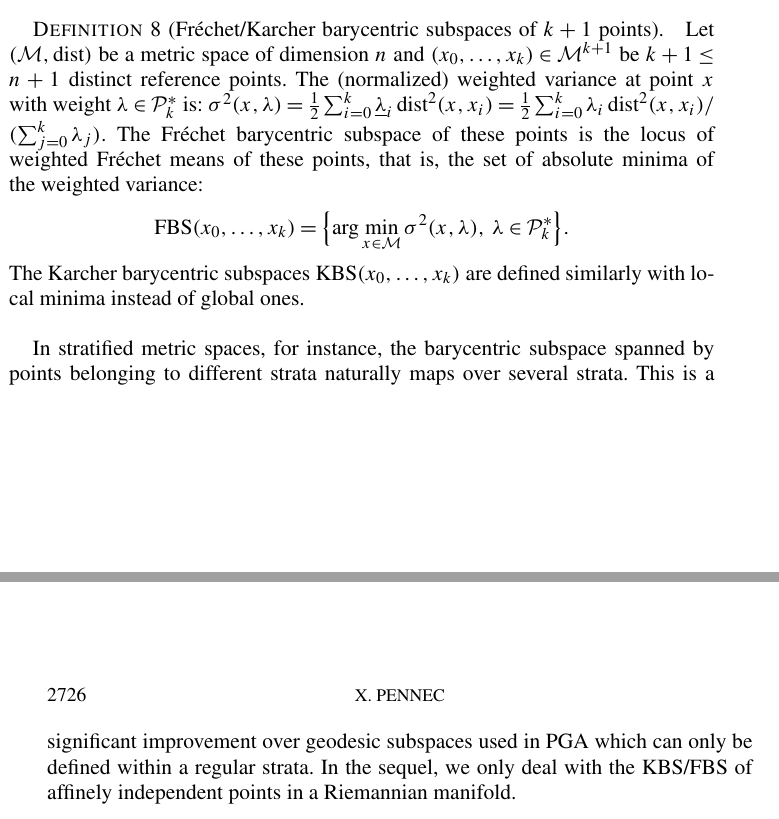
\includegraphics[width=1\linewidth]{figs/pennec2018-sec4-1.PNG}}
\vspace{1em}
}
Nessa definição, o autor nos define os espaços baricêntricos de Fréchet ou Karcher. Essencialmente, ambos os espaços compostos pelos pontos que minimizam a variança, com a diferença em que no espaço de Fréchet contém apenas mínimos globais, quanto a de Karcher considera tembém os mínimos locais. A variânça nesses espaços é definida pela distância geodésica por que ela tem a capacidade de trazer tanto a média quanto a váriança para um ponto que pertence a variedade.
{
\vspace{1em}
\frame{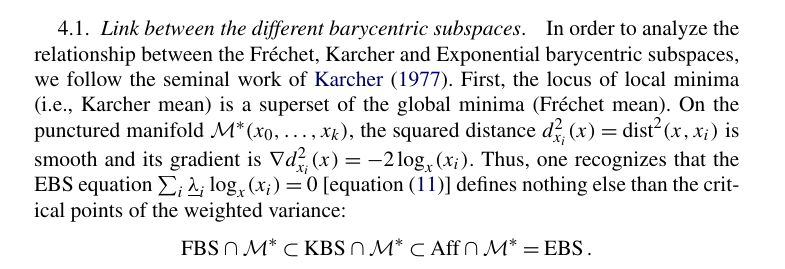
\includegraphics[width=1\linewidth]{figs/pennec2018-sec4-2.PNG}}
\vspace{1em}
}
Aqui o autor mostra a relação entre os espaços de Karcher, Fréchet  e afim. O $\mathcal{M}^*$ é o conjunto de dados cujo a distância geodésica tem por gradiente o mapeamento logaritmico. as interseções dos espaços aos conjuntos de dados são simples de se entender: O $FBS \cap \mathcal{M}^*$ é o conjunto de pontos que minimizam globalmente o conjunto de dados, $KBS \cap \mathcal{M}^*$
é o conjunto com todos os mínimos locais, $Aff \cap \mathcal{M}^*$ é o próprio mapeamento exponencial do conjunto de dados. Como a média de Fréchet é um caso específico da média de Karcher e a média de Karcher pega apenas alguns pontos do espaço afim. Então é natural que a relação $FBS \cap \mathcal{M}^* \subset KBS \cap \mathcal{M}^* \subset Aff \cap \mathcal{M}^* = EBS$

\section{Commented and Expanded Section 5: Properties of the barycentric
subspaces}

{
\vspace{1em}
\frame{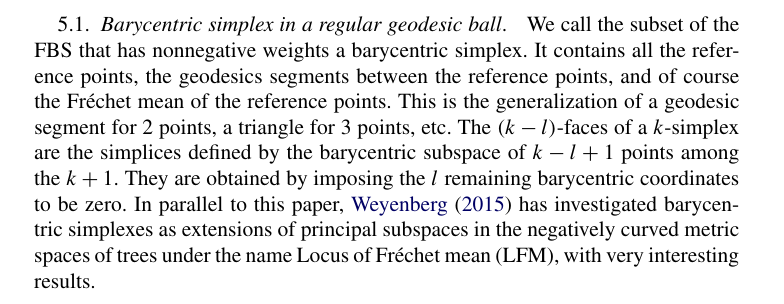
\includegraphics[width=1\linewidth]{figs/pennec2018-sec5-1.PNG}}
\vspace{1em}
}
Aqui o autor propõe pegar um subconjunto positivo do FBS, que pega todas as distância geodésicas dos pontos e da média de Fréchet. a partir disto, ele cria um espaço baricêntrico 
{
\vspace{1em}
\frame{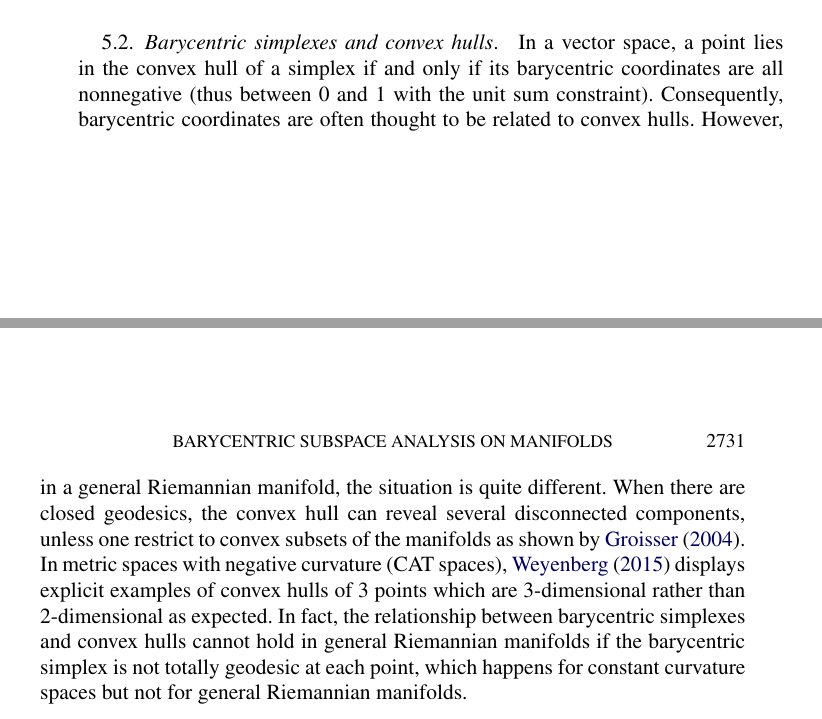
\includegraphics[width=1\linewidth]{figs/pennec2018-sec5-2.PNG}}
\vspace{1em}
}
{
\vspace{1em}
\frame{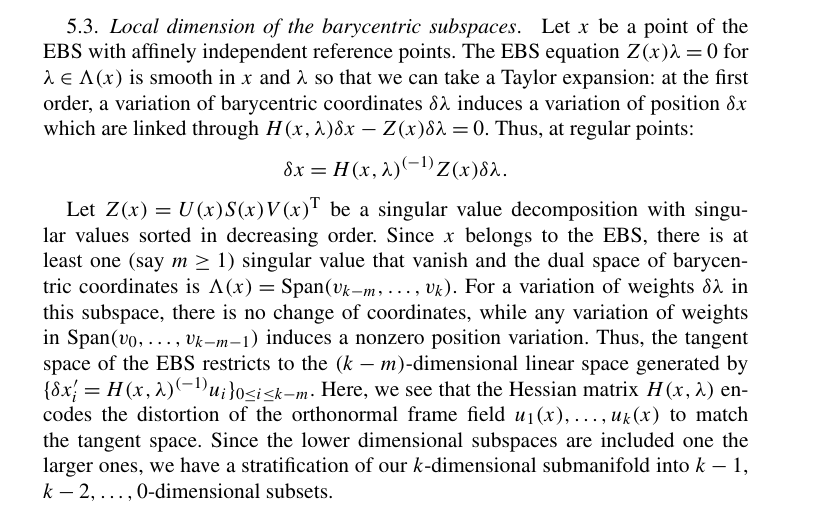
\includegraphics[width=1\linewidth]{figs/pennec2018-sec5-3.PNG}}
\vspace{1em}
}
{
 
{
\vspace{1em}
\frame{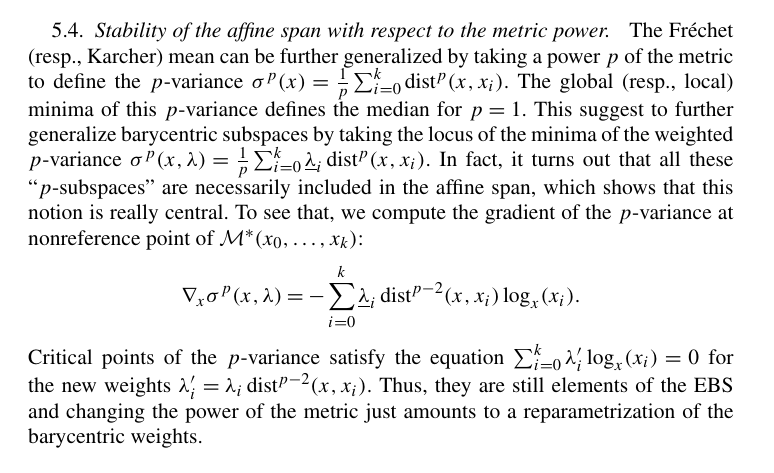
\includegraphics[width=1\linewidth]{figs/pennec2018-sec5-5.PNG}}
\vspace{1em}
}
{
\vspace{1em}
\frame{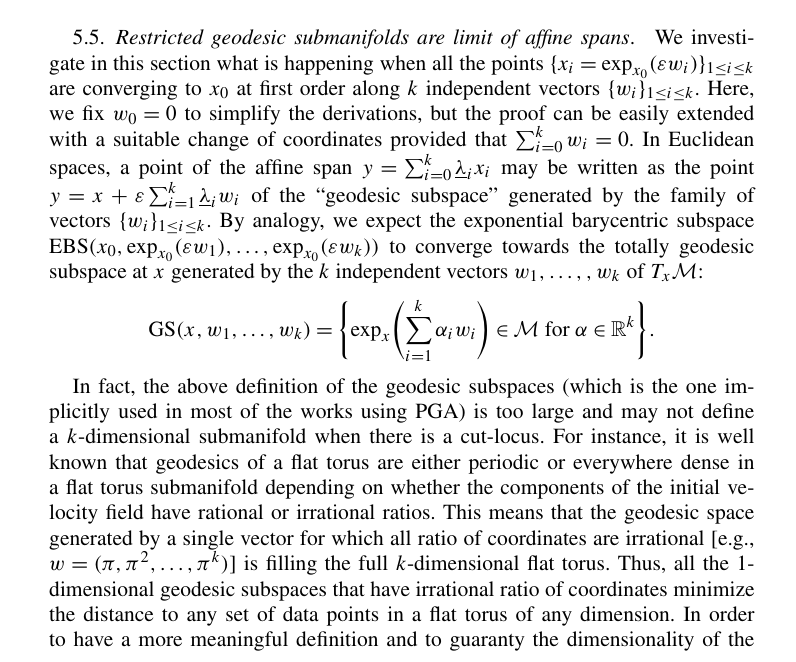
\includegraphics[width=1\linewidth]{figs/pennec2018-sec5-6.PNG}}
\vspace{1em}
}
{
\vspace{1em}
\frame{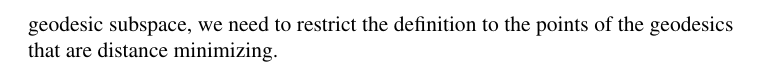
\includegraphics[width=1\linewidth]{figs/pennec2018-sec5-7.PNG}}
\vspace{1em}
}

\section{Commented and Expanded Section 6: Barycentric subspace analysis}


{
\vspace{1em}
\frame{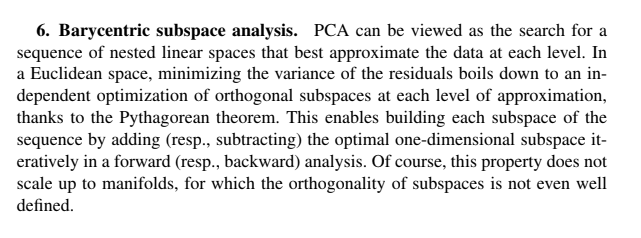
\includegraphics[width=1\linewidth]{figs/pennec2018-sec6-1.PNG}}
\vspace{1em}
}
Nesta introducao, diz que a PCA é uma busca por uma sequencia de espaços lineares agrupados que melhor aproximam a informação a cada nível. Uma boa tradução para esta primeira frase é que a PCA, busca as retas que pegam melhor os pontos de um grupo de pontos, isto é feito, pelo que ele diz, graças ao teorema de Pitágoras é possivel criar uma otimização do espaço residual. O teorema de Pitágoras é o quadrado da distância entre os pontos e a curva modelada em um espaço linear. Porém quando extendemos esta análise ao mundo das variedades, o uso do quadrado da distância euclidiana passa a não funcionar já que estamos trabalhando em um espaço simbólico e tal uso seria possível apenas atribuindo coordenadas a variedade, tornando ela linear. Então nesta seção o autor busca encontrar uma maneira de fazer essa PCA extender-se as variedades

{
\vspace{1em}
\frame{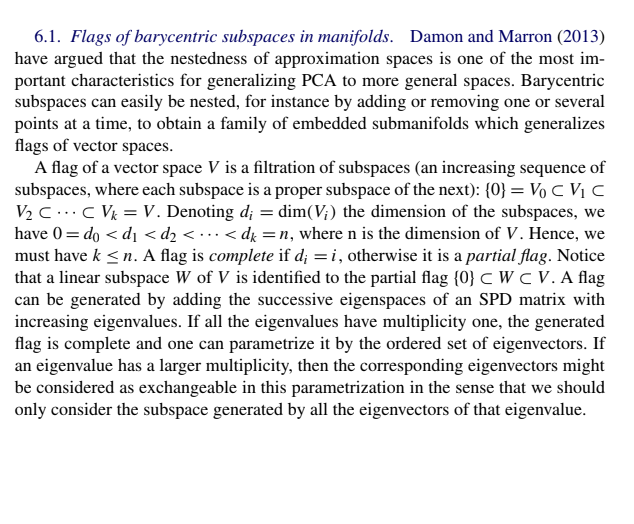
\includegraphics[width=1\linewidth]{figs/pennec2018-sec6-2.PNG}}
\vspace{1em}
}

Neste trecho, o autor busca mostrar as primeiras fases disso é estabelecer o as bases do que ocorre inicialmente no espaço euclidiano. Para isso ele usa a noção de flag. Além disso ele nos apresenta as seguintes características: A flag pode ser formada pelos autoespaço de dimensão i, se os autosvalores relacionados aos autovetores que compõem o autoespaço forem de multiplicidade 1 e os autovetores formarem uma matriz de um sistema linear possível e determinado, $Dim(V_i)=d_i=i$ que é dito que a flag é completa. Isso, em termos geométricos significa que a flag completa é composta por pontos em todo $V_i$, caso seja completo são independentes e a matriz de autoespaço é possui posto completo. Caso a possuamos autovalores de de multiplicidade maior que 1, as soluções são geométricamente como retas, planos, hiperplanos em $V_i$ e o posto da matriz do autoespaço é menor que $i$ \draftnote{Gabriel: Isso é facilmente percebido, mas eu não sei se fica bom comentar isso}.

{
\vspace{1em}
\frame{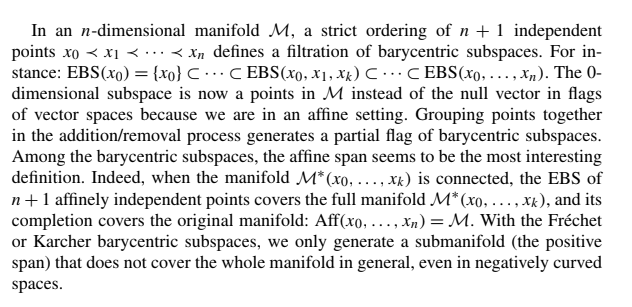
\includegraphics[width=1\linewidth]{figs/pennec2018-sec6-3.PNG}}
\vspace{1em}
}
Agora ele passa a analisar na variedade. Para isso ele redefine a noção de flag utilizando subespaços baricêntricos exponenciais. A abordagem utilizando SBE (tradução livre do EBS) para escrever a "flag generalizada" é similar a de cima porém o resultado gerado com ele é que possamos cobrir a variedade por completo a partir do mapeamento exponencial urilizado no SBE. Como o mapeamento exponencial que ele utiliza é a tradução do espaço da variedade centrada na origem somando um espaço afim, ele consegue chegar a $Aff(x_0,...,x_k) = \mathcal{M}$. Por fim ele cria uma subvariedade com os pontos de mínimo pela média de Karcher ou Fréchet.

{
\vspace{1em}
\frame{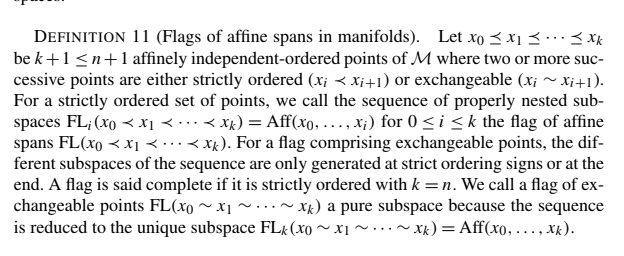
\includegraphics[width=1\linewidth]{figs/pennec2018-sec6-4.PNG}}
\vspace{1em}
}
Aqui o autor apenas formaliza o que foi dito anteriormente e nos mostra como a nova definição de flag pode ser criada com o uso do espaço afim \draftnote{Gabriel: Talvez haja uma maneira melhor de expandir isso}
{
\vspace{1em}
\centering
\frame{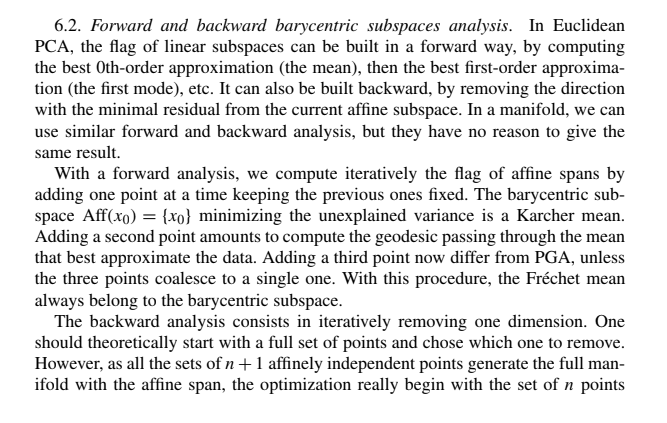
\includegraphics[width=1\linewidth]{figs/pennec2018-sec6-5.PNG}}
\vspace{1em}
}
Neste trecho o autor apenas estabelece as diferenças da PCA no espaço euclidiano e a PCA proposta. No espaço euclidiano, quando queremos propor o encontro do mínimo, podemos utilizar a média, a variânça e outras técnicas para encontrar o mínimo de erro possível dos dados, porém em se tratando de variedades essa média é a média de Karcher ou Fréchet a depender do uso. Essas médias buscam o mínimo da distância geodésica ao quadrado, tornando a PCA proposta possível para um problema no espaço da variedade. Outra coisa que o autor aborda é a possibilidade de criar além da análise avançada que é feita no processo da alínea anterior, tembém há a criação das flags por meio "recuado", onde nela, é retirado a direção que otimiza o conjunto de pontos da variedade até chegar ao ponto ótimo pela média de Karcher.

{
\vspace{1em}
\centering
\frame{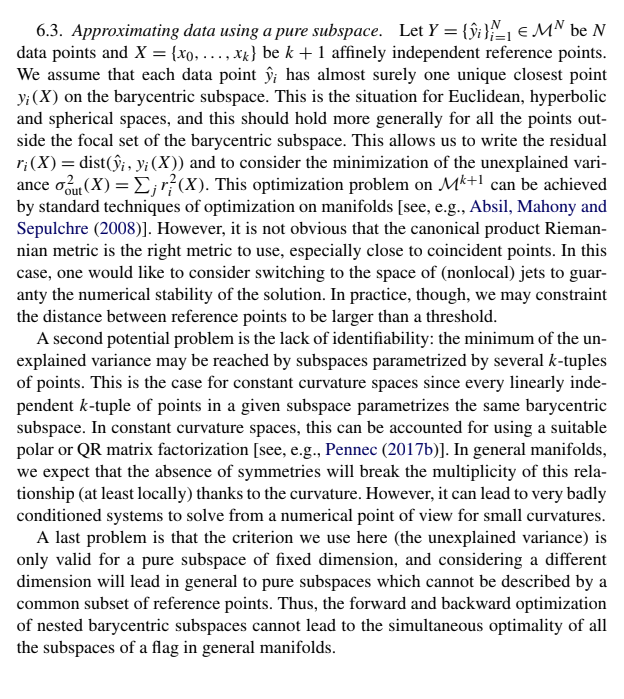
\includegraphics[width=1\linewidth]{figs/pennec2018-sec6-6.PNG}}
\vspace{1em}
}

Neste trecho o autor mostra alguns procedimentos de como fazer essa aproximação utilizando os resíduos como a distância dos pontos coletados na variedade e uma função $y$ que mapeia os pontos da variedade com base no conjunto de dados e mostra que a variança ao quadrado dos dados é a soma dos quadrados das distâncias geodésicas dos dados e nos mostra que isso pode nos fornecer respostas incorretas devido ao fato de que podem haver varianças parametrizadas por outras subvariedades, que provém da existência de múltiplos caminhos geodésicos, o fato de que utilizar subespaços de dimensão fixa podem tendenciar a PCA, por conta da falta de uma dimensão ela pode considderar pontos "errados" como sendo certos e o fato de que nem sempre a métrica riemmaniana senm sempre ser a melhor opção, isso porque podemos ficar presos a mínimos locais quando queremos ter uma visão global do problema.

\section{Commented and Expanded Section 7: Discussion}

Nesta seção o autor resume todo o conteúdo que nos foi apresentado ao longo do texto e nos 

\section{Commented and Expanded Appendix: Proof of Theorem 8}
{
\vspace{1em}
\frame{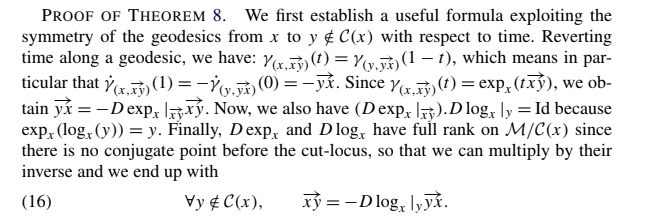
\includegraphics[width=1\linewidth]{figs/pennec2018-sec8-1.PNG}}
\vspace{1em}
}
\sout{Nesta seção o autor nos provém primeiramente com uma função que pega e leva de
$x  a y \notin C(x)$ em respeito ao tempo e ele também nos informa que
revertendo o tempo ao longo da geodésica, tem-se
$\gamma_{(x,\overrightarrow{xy})}(t)=\gamma_{(y,\overrightarrow{yx})}(1-t)$, e
ele também diz que em
$\dot{\gamma_{(x,\overrightarrow{xy})}}(1)=\dot{\gamma_{(y,\overrightarrow{yx})}}(0)=-\overrightarrow{yx}$.
Isto que o autor faz em um espaço geodésico é similar a uma abordagem em uma
parametrização em um espaço euclidiano $x(t)=x_{0}t+(1-t)x_{1}$ e pelo que
pode-se entender $\overrightarrow{xy}$ é o vetor distância de $x$ a $y$,
portanto faz sentido que $\overrightarrow{xy}=-\overrightarrow{yx}$. Então ele
define que $\gamma_{(x,\overrightarrow{xy})}(t)=exp_{x}(t \overrightarrow{xy})$,
temos $\overrightarrow{yx}=-D
exp_{x}|_{\overrightarrow{xy}}\overrightarrow{xy}$\draftnote{Gabriel's note: Por
favor expandir isso!}. Pelo fim do parágrafo é definido que $(D
exp_{x}|_{\overrightarrow{xy}}\overrightarrow{xy})D log_{x}|_{y} = Id$ pelo fato
de $exp_{x}(log_{x}(y))=y$ e finalmente ele considera que se tanto $Dexp_{x}$
quanto $Dlog_{x}$ possuírem o posto aquivalente ao expaço quociente da variedade
com o domínio em x, podemos criar uma função inversa como descrito na equação
(16).}
Neste parágrafo o autor faz uma extensão da simetria das geodésicas em relação a um tempo $t$. Essa construção é possível graças ao fato de ser variedade riemmaniana completa. Após isto, ele define a relação de simetria em termos da geodésica normalizada e mostra que em um tempo particular $t=1 \rightarrow \dot{\gamma_{(x,\overrightarrow{xy})}}(1)=\dot{\gamma_{(y,\overrightarrow{yx})}}(0)=-\overrightarrow{yx}$.\draftnote{Gabriel: Esse ponto em cima é a notação de derivada para o autor? Não ficou claro} 
Como a função da geodésica normalizada é definida pelo mapeamento exponencial no ponto $x$, a derivada 
{
\begin{equation}
	\frac{d\gamma_{(x,\overrightarrow{xy})}(t)}{dt} = exp_{x}(t \overrightarrow{xy})\overrightarrow{xy}
\end{equation}
}
Após isso ele procura define que a funcao inversa ao mapeamento exponencial que eh o mapeamento logaritmico e diz $D(exp_{x}|_{\overrightarrow{xy}})Dlog_{x}|_y=Id$. Essa relacao aparece quando se aplica a $D$ em $exp_{x}(log_x(y))$ onde vai aparecer a regra da cadeia da derivada.  

{
\vspace{1em}
\frame{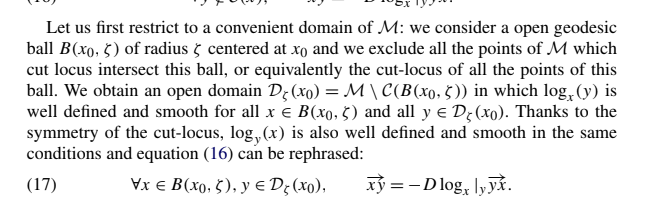
\includegraphics[width=1\linewidth]{figs/pennec2018-sec8-2.PNG}}
\vspace{1em}
}

\sout{ No segundo parágrafo, tendo as funções definidas ele considera uma bola
aberta geodésica $B(x_0,\zeta)$ e se for construído um domínio $D_{\zeta}=M \\
C(B(x_0,\zeta)$ em q $log_{x}(y)$ seja suave e bem definida na bola e para todo y
em D, a simetria é preservada, portanto (16) pode ser reescrito como (17)}
Aqui o autor restringe o domínio criando uma bola aberta de raio $\zeta$ e centro $x_0$
e fez um novo domínio que é a variedade sem os pontos de corte locais em que o mapeamento logaritmico é bem definido e suave ao longo de $B$ e $\mathcal{D}$. O fato do mapeamento exponencial ser simétrico e o corte local ser o mapeamento exponencial, o mapeamento logaritmico também compartilha das mesma propriedades de suavidade, portanto a equação (16) é válida no domínio $\mathcal{D}$, possibilitando sua reescrita na equação (17)

{
\vspace{1em}
\frame{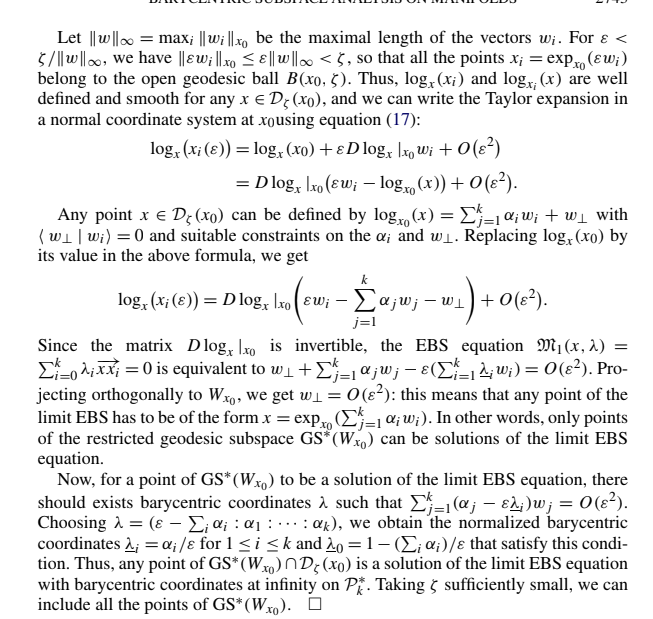
\includegraphics[width=1\linewidth]{figs/pennec2018-sec8-3.PNG}}
\vspace{1em}
}

Nesta última parte, o autor junta as ideias anteriores, primeiro definindo um
tamanho máximo dos vetores $w_i$ que compõem o corte local e definindo um erro
menor que o raio da bola aberta geodésica de raio $\zeta$. Ele usa isso para provar que todos os pontos desta bola fazem parte do corte local em $x0$. Ele também mostra que se conseguirmos criar um espaço dual de $x$ e $x_i$ onde, para todo $x \in \mathcal{D}$, expansão logaritmica de $x_i$ em torno de $x$ e vice-versa são bem definidas e suaves em $\mathcal{D}$, ele escreve uma expansao em série de Taylor em torno de $x_0$. Sendo asim

{
\begin{equation}
	x_i(\epsilon) = x_0+\epsilon D w_i +O(\epsilon^2)
\end{equation}
} 
aplicando o mapa logaritmico temos a equacao dada \draftnote{Gabriel: Como escrever isso melhor?}
%\section{Commented and Expanded Supplementary Material}


\bibliographystyle{ieeetr}
\bibliography{refs}
%bib/edge-linking,bib/deformable,bib/medical,bib/graphics,bib/texture,bib/imaging,bib/tracking,bib/shape-papers,bib/bib-header,bib/video,bib/math-books,bib/math,bib/psych-books,bib/metric,bib/edge,bib/leymarie_pami_scaffold,bib/vision-books,bib/vision,bib/nn-search,bib/multidimscaling,bib/psychophysics,bib/indexing,bib/segmentation,bib/image-databases,bib/shape-matching,bib/neuro,bib/skeleton,bib/skeleton2D,bib/aspect-graphs,bib/recognition,bib/surface-networks,bib/ridge,bib/proceedings,bib/perceptual-grouping,bib/continuation,bib/graph-matching-2,bib/cooper}
%DAMON, J. and MARRON, J. S. (2013). Backwards principal component analysis and principal nested relations. J. Math. Imaging Vision 50 107–114. MR3233137
%\input{paper.bbl}
% Le, Huiling. “A DIFFUSION PROCESS ASSOCIATED WITH FRÉCHET MEANS.” The Annals of Applied Probability, vol. 25, no. 6, 2015, pp. 3033–3046., www.jstor.org/stable/24521650. Accessed 30 June 2021.
%WILSON, R. C., HANCOCK, E. R., PEKALSKA, E. and DUIN, R. P. W. (2014). Spherical and hyperbolic embeddings of data. IEEE Trans. Pattern Anal. Mach. Intell. 36 2255–2269.
%Marc Arnaudon, Frédéric Barbaresco, Le Yang. Medians and means in Riemannian geometry: existence, uniqueness and computation. 2011. ffhal-00640626

% Assinaturas:
%\newpage
%\ \\\vspace{7cm}
%\center $\overline{\ \ \ Ricardo\ Fabbri\ \ \ }$
%\ \\\vspace{4cm}
%\center $\overline{\ \ \ Luciano\ da\ Fontoura\ Costa\ \ \ }$
\end{document}
